\documentclass[14pt, aspectratio=169]{beamer}
\usetheme{Frankfurt}
\usecolortheme{default}
\usefonttheme{professionalfonts}

\usepackage{cmap} % нормальное копирование, поиск в PDF
\usepackage[T2A]{fontenc} % кодировка
\usepackage[utf8]{inputenc} % кодировка исходного текста
\usepackage[english,russian]{babel} 
\usepackage{graphicx}
\usepackage{tikz, pgfplots} 
\usetikzlibrary{positioning}
\setbeamertemplate{caption}[numbered]
\usepackage{amsmath}


\title{Численное решение задачи двухфазной фильтрации}
\author{Самигуллин Линар}
\institute{МФТИ, Роснефть}
\date{\today}

\begin{document}

\maketitle

\begin{frame} {Содержание}

    \tableofcontents

\end{frame}

\section{Задача}

\begin{frame} {Постановка задачи}

    \begin{columns}
        \column{0.5\textwidth} 
        В насыщенную нефтью пористую среду закачивают воду.

        Необходимо рассчитать поле водонасыщенности в момент времени t.

        \begin{figure}
            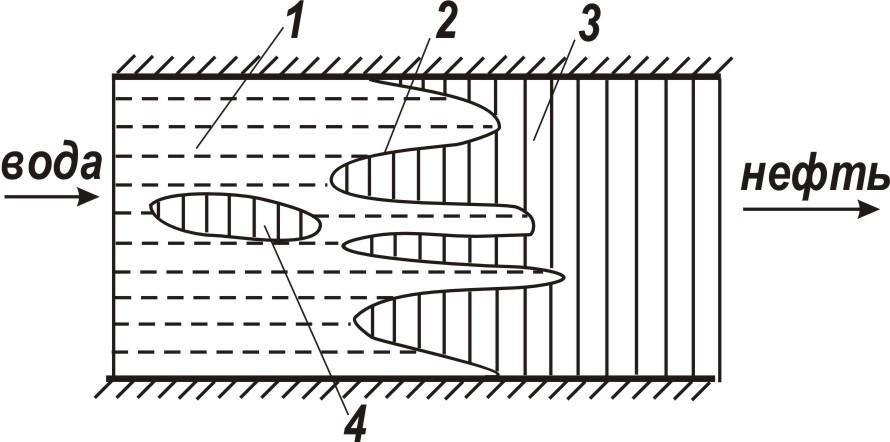
\includegraphics[width=0.7\linewidth]{scheme-image-filtration.jpg}
        \end{figure}

        \column{0.5\textwidth} Допущения:
            \begin{itemize}
                \item Пористая среда и жидкости несжимаемы
                \item Жидкости несмешивающиеся
                \item Пренебрегаем капиллярным давлением
                \item Рассматриваем одномерный случай без гравитационных сил
            \end{itemize}
    \end{columns}

\end{frame}

\section{Уравнения}

\begin{frame} {Уравнение неразрывности}

    \begin{block}{Уравнение неразрывности}
    $
    \frac{\partial r_{\alpha} }{\partial t} + \nabla \cdot \left( r_{\alpha} \vec{v}_{\alpha} \right) = 0,
    $
    \end{block}

    В нашем случае для воды:
    $
    r_1 = \rho_{1} S \phi 
    $,

    для нефти: $
    r_2 = \rho_{2} (1 - S) \phi 
    $,
    где $S$ - водонасыщенность.

    Подставляя, получим 2 уравнения:
    
    $$
    \frac{\partial ( \rho_{1} S \phi ) }{\partial t} + \nabla \cdot \left( \rho_{1} S \phi \vec{v}_{1} \right) = 0
    $$
    $$
    \frac{\partial \left( \rho_{2} (1 - S) \phi \right) }{\partial t} + \nabla \cdot \left( \rho_{2} (1 - S) \phi \vec{v}_{2} \right) = 0
    $$

\end{frame}

\begin{frame}{Уравнение неразрывности}
    Заметим, что $\vec{W}_{\alpha} = S_{\alpha} \phi \vec{v}_{\alpha}$, - вектор скорости фильтрации жидкости $\alpha$, тогда:
    $$
    \frac{\partial ( \rho_{1} S \phi ) }{\partial t} + \nabla \cdot \left( \rho_{1} \vec{W}_{1} \right) = 0,
    $$

    Так как пористая среда и жидкости несжимаемы, тогда:
    
    $$
    \phi \frac{\partial S }{\partial t} + \nabla \cdot \vec{W}_{1} = 0, $$ 
    
\end{frame}

\begin{frame}{Уравнение неразрывности}
    Просуммировав уравнения для нефти и воды, получим:
    $$
    \nabla \cdot \left( \vec{W}_{1} + \vec{W}_{2} \right)= 0
    $$

    В одномерном плоскопараллельном случае:
    $$
    \phi \frac{\partial S }{\partial t} + \frac{\partial W_{1}}{\partial x} = 0
    $$
    $$
    \frac{\partial}{\partial x} \left( W_1 + W_2 \right) = 0
    $$
    
\end{frame}

\begin{frame}{Уравнение движения}
    \textbf{Обобщенный закон Дарси}, пренебрегая капиллярным давлением:

    $$
    \vec{W}_{\alpha} = - k \frac{f_{\alpha}(S_{\alpha})}{\mu_{\alpha}} \nabla P
    $$

    В одномерном случае:
    $$
    W_{\alpha} = - k \frac{f_{\alpha}(S_{\alpha})}{\mu_{\alpha}} \frac{\partial P}{\partial x}
    $$

\end{frame}


\begin{frame}{Относительные фазовые проницаемости}
    
    \begin{figure}
        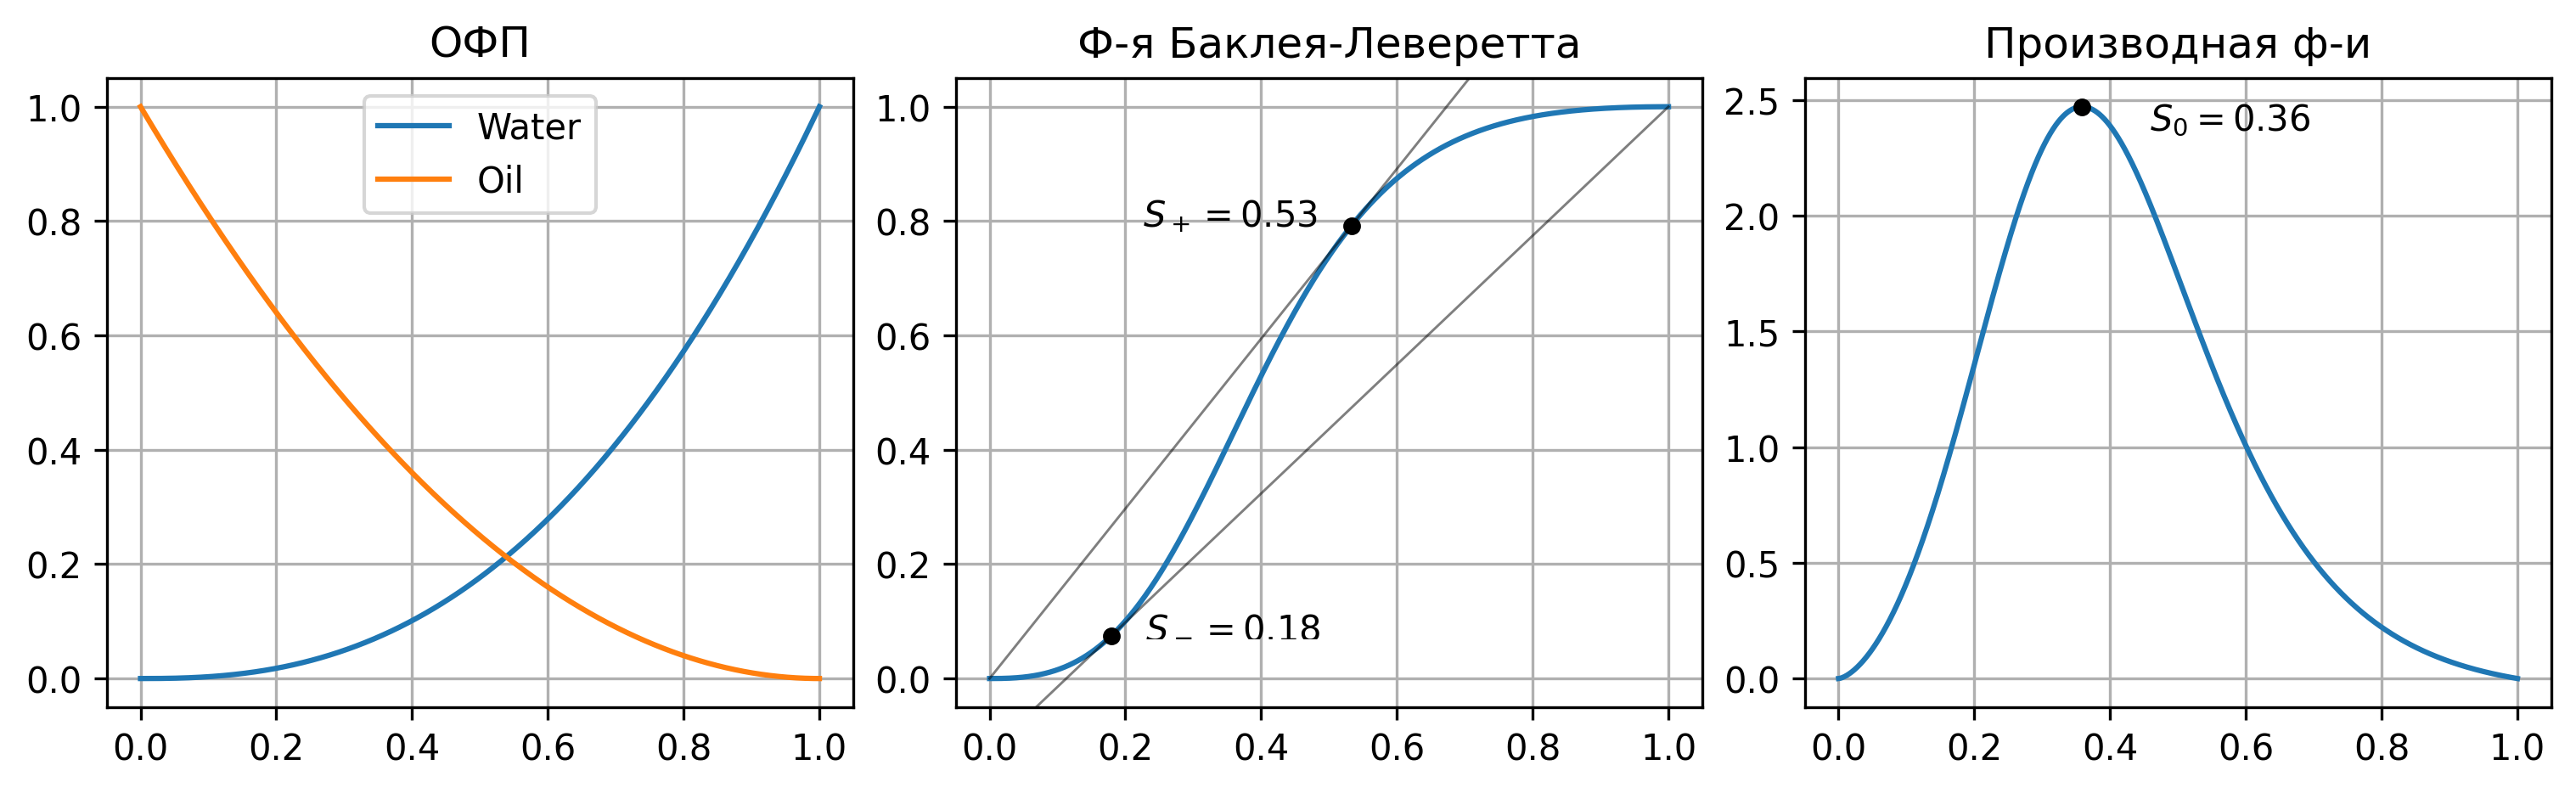
\includegraphics[width=0.9\linewidth]{buckley-leverett-plot.png}
    \end{figure}

    \begin{columns}
        \column{0.3\textwidth}
        ОФП по Corey:

        $
        f_1(S) = S^{n}$ \\ $
        f_2(S) = (1 - S)^{m}
        $
        \column{0.5\textwidth}
        Функция Баклея-Леверетта:

        $
        b(S) = \frac{f_1(S)}{f_1(S) + \frac{\mu_1}{\mu_2} {f_2(S)}}
        $
    \end{columns}
    

\end{frame}

\section{Решения}
\subsection{Точное решение}

\begin{frame} {Точное решение}

    \begin{block}{Характеристическая скорость}
    $$
    U(S) = \frac{W}{\phi} \frac{d b(S)}{d S}
    $$
    \end{block}

    \begin{figure}
        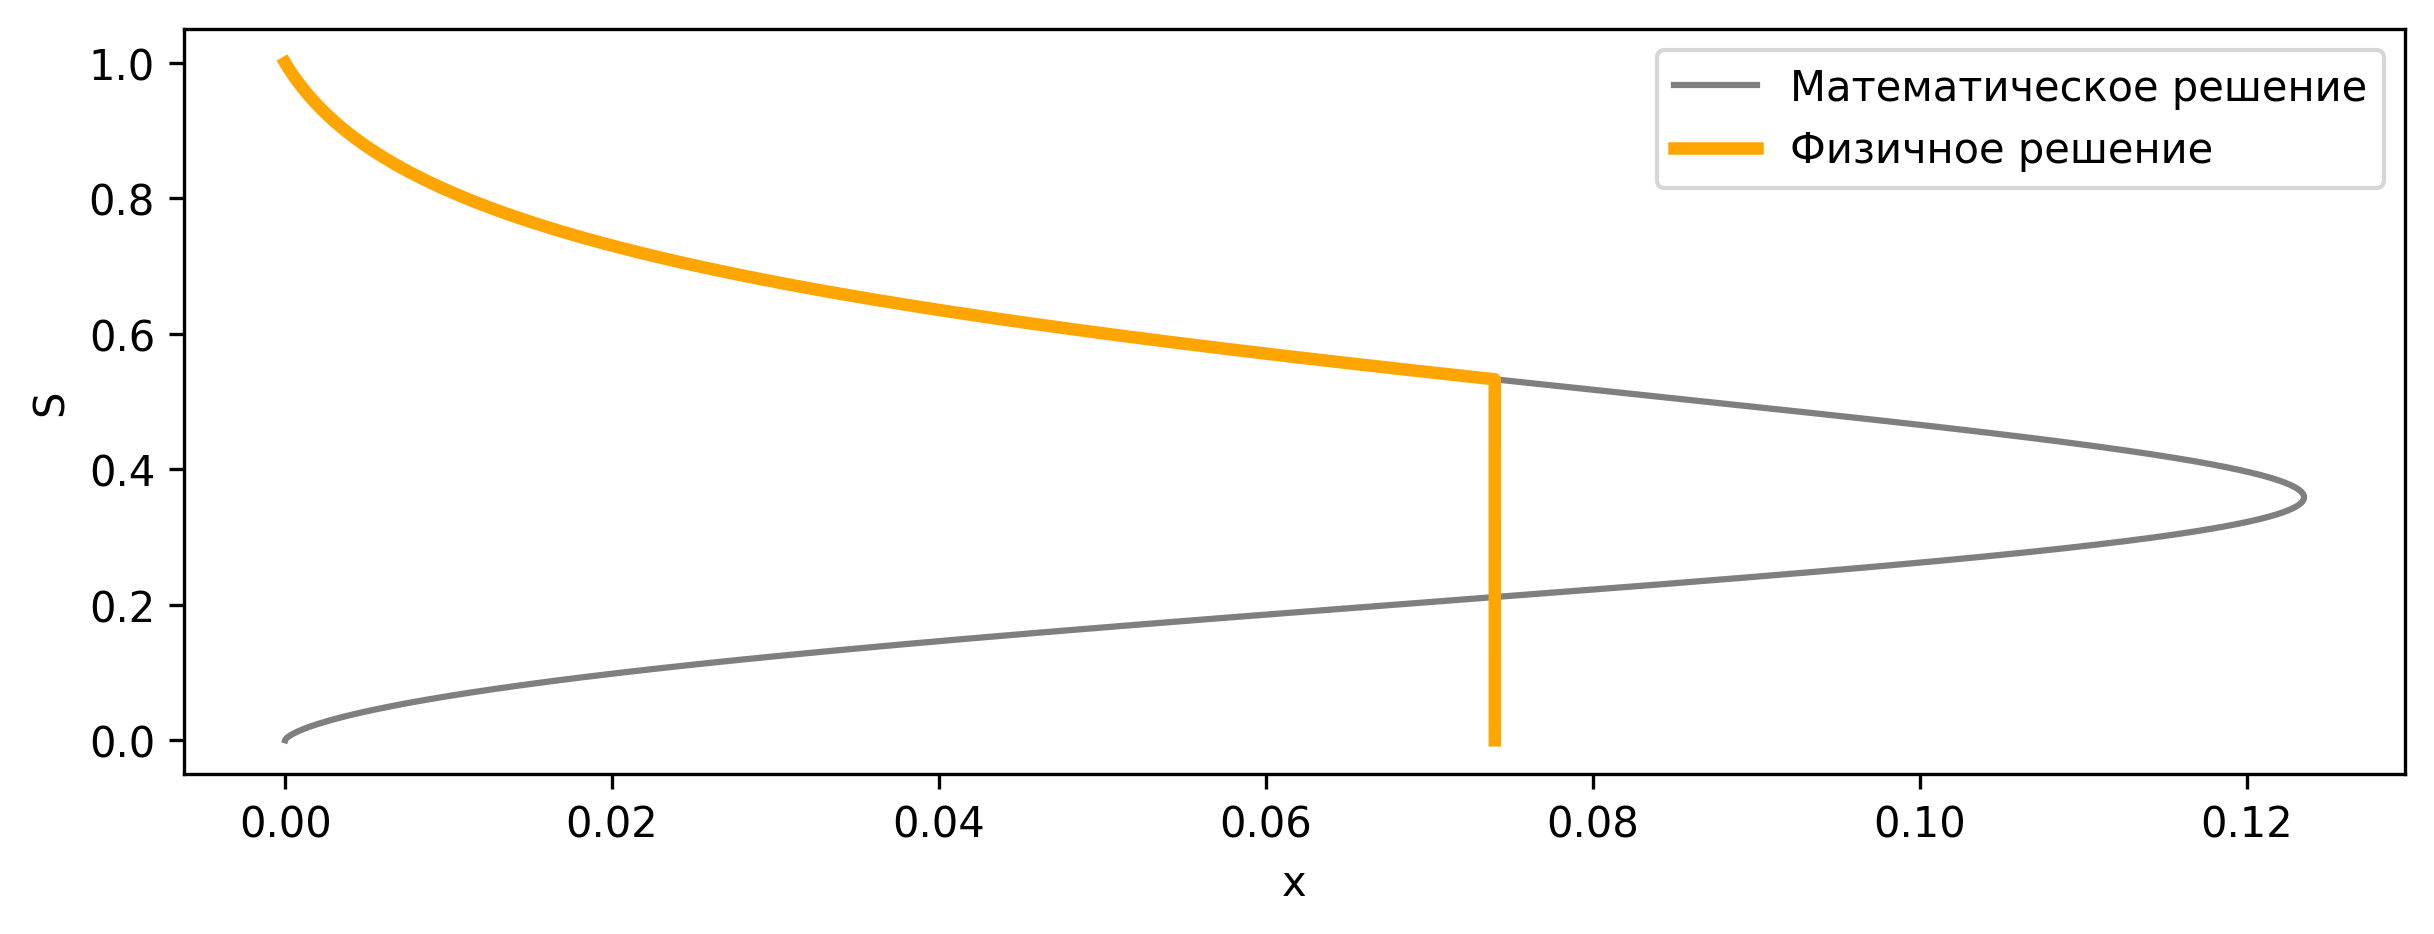
\includegraphics[width=0.7\linewidth]{characteristic-solution.png}
    \end{figure}

\end{frame}

\subsection{Численные решения}

\begin{frame} {Обзор методов решения}

    \begin{itemize}
        \item Численное решение гиперболического уравнения относительно $S$, c граничным условием $W(t)$ \\ $$
        \frac{\partial S }{\partial t} + \frac{W}{\phi} \frac{\partial b(S)}{\partial x} = 0
        $$
        
        \item Численное решение сиcтемы уравнений относительно $S$ и $P$, с граничным условием $P(t)$
    \end{itemize}

    \begin{equation*}
        \begin{cases}
            \frac{\partial S }{\partial t} + \frac{1}{\phi} \frac{\partial W_1}{\partial x} = 0\\
            \frac{\partial}{\partial x} \left[ \frac{\partial P}{\partial x} \left( \frac{f_1(S)}{\mu_1} + \frac{f_2(S)}{\mu_2} \right) \right] = 0
        \end{cases}
    \end{equation*}
    

\end{frame}


\subsubsection{Upwind}
\begin{frame} {Разностная противопоточная схема}

    \begin{columns}
        \column{0.75\textwidth}
        $$
        \frac{\partial S }{\partial t} + \frac{W}{\phi} \frac{\partial b(S)}{\partial x} = 0
        $$
        $$
        \frac{S_{i}^{n+1} - S_{i}^{n}}{\tau} + \frac{W}{\phi} \frac{b(S_{i}^n) - b(S_{i-1}^n)}{h} = 0, \hspace{0.5cm} W>0
        $$
        $$
        \frac{S_{i}^{n+1} - S_{i}^{n}}{\tau} + \frac{W}{\phi} \frac{b(S_{i+1}^n) - b(S_{i}^n)}{h} = 0, \hspace{0.5cm} W<0
        $$
        \begin{block}{}
            $$
            S_{i}^{n+1} = S_{i}^{n} - \frac{W \tau}{\phi h} \left( b(S_{i}^n) - b(S_{i-1}^n) \right)
            $$
        \end{block}
        \column{0.25\textwidth}
        \begin{center}
            \resizebox{3cm}{!}
            {
            \begin{tikzpicture}
                \draw[ultra thin] (0,0) grid (3,3);
                \draw[thick] (1,1) -- (2,1);
                \draw[thick] (2,1) -- (2,2);
                \filldraw[red] (2, 2) circle (0.05);
                \filldraw[black] (2, 1) circle (0.05);
                \filldraw[black] (1, 1) circle (0.05);
                
                \draw[->][thick] (0.5, 1.5) -- (1.5, 1.5);
                \draw node at (0.6, 1.8) {\small \textit{flow}};
    
                \draw node at (2.5, 2.3) {\small $S_i^{n+1}$};
                \draw node at (2.3, 0.7) {\small $S_i^{n}$};
                \draw node at (0.6, 0.7) {\small $S_{i-1}^{n}$};
            \end{tikzpicture}
            }
        \end{center}
    
        \begin{center}
            \resizebox{3cm}{!}
            {
            \begin{tikzpicture}
                \draw[ultra thin] (0,0) grid (3,3);
                \draw[thick] (1,1) -- (2,1);
                \draw[thick] (1,1) -- (1,2);
                \filldraw[red] (1, 2) circle (0.05);
                \filldraw[black] (1, 1) circle (0.05);
                \filldraw[black] (2, 1) circle (0.05);
                
                \draw[->][thick] (2.5, 1.5) -- (1.5, 1.5);
                \draw node at (2.4, 1.8) {\small \textit{flow}};
    
                \draw node at (0.55, 2.3) {\small $S_i^{n+1}$};
                \draw node at (2.5, 0.7) {\small $S_{i+1}^{n}$};
                \draw node at (0.6, 0.7) {\small $S_{i}^{n}$};
            \end{tikzpicture}
            }
        \end{center}
    \end{columns}

\end{frame}

\begin{frame} {Результат \textbf{upwind} схемы}

    \begin{figure}
        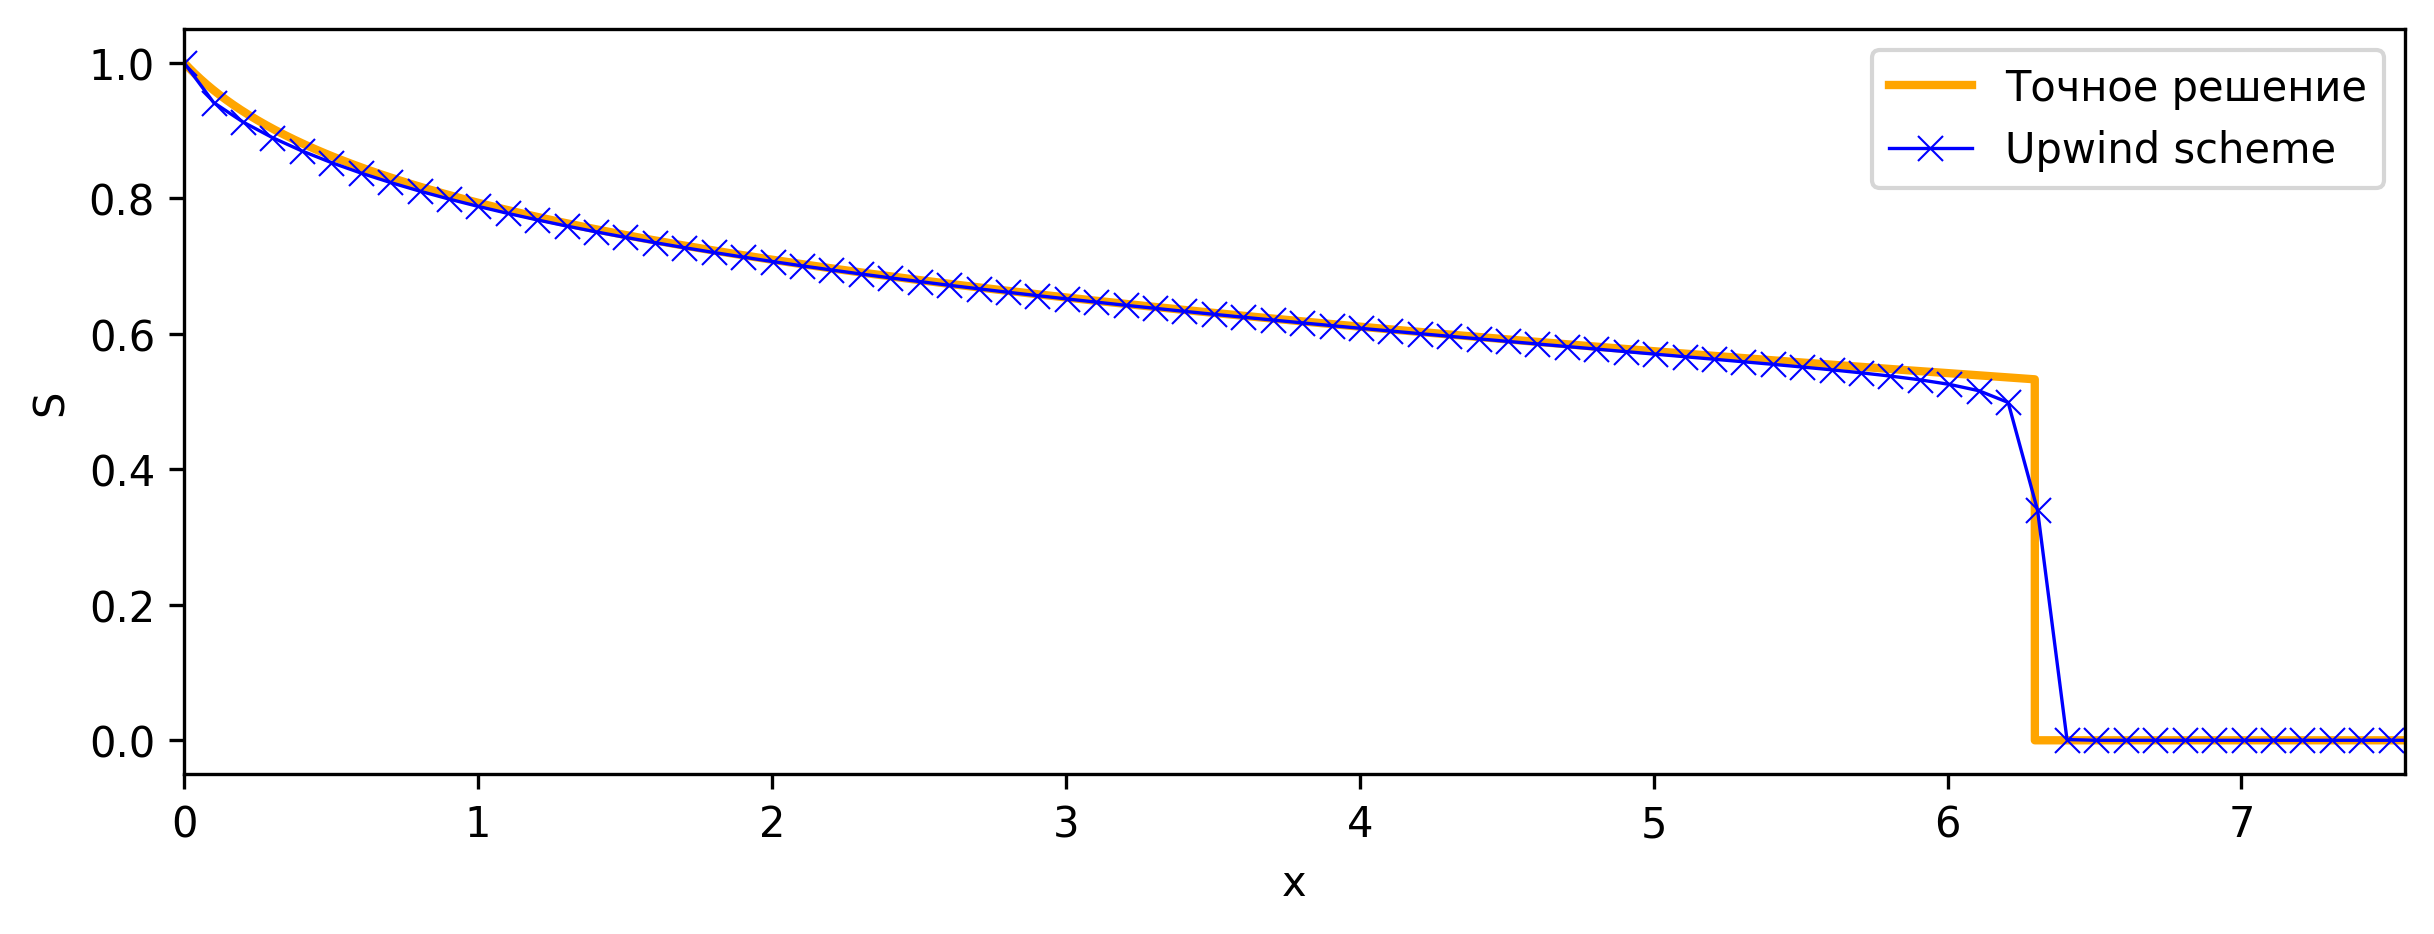
\includegraphics[width=\linewidth]{upwind-solution-0.png}
        \caption{Поле водонасыщенности по противопоточной схеме}
    \end{figure}

\end{frame}

\subsubsection{IMPES}

\begin{frame} {Метод \textbf{IMPES}}

    Алгоритм \textbf{IM}plicit\textbf{P}ressure\textbf{E}xplicit\textbf{S}aturation:

    \begin{enumerate}
        \item Находим \textbf{неявно} поле $P^n$ по $S^n$
        \item По найденному полю $P^n$ находим \textbf{явно} $S^{n+1}$
    \end{enumerate}
    
\end{frame}

\begin{frame} {Уравнение для давления}

    $$
    \frac{\partial}{\partial x} \left[ \frac{\partial P}{\partial x} \left( \frac{f_1(S)}{\mu_1} + \frac{f_2(S)}{\mu_2} \right) \right] = 0
    $$

    $$
    \frac{\partial^2 P}{\partial x^2} \left( \frac{f_1(S)}{\mu_1} + \frac{f_2(S)}{\mu_2} \right) + \frac{\partial P}{\partial x} \frac{\partial}{\partial x}\left(  \frac{f_1(S)}{\mu_1} + \frac{f_2(S)}{\mu_2} \right) = 0
    $$
    \\

    Пусть $\alpha = \left( \frac{f_1(S)}{\mu_1} + \frac{f_2(S)}{\mu_2} \right)$, тогда:

    $$
    \frac{\partial^2 P}{\partial x^2} \alpha + \frac{\partial P}{\partial x} \frac{\partial \alpha}{\partial x} = 0
    $$

\end{frame}

\begin{frame}{Дискретизация}
    На $n$-м слое:
    $$
    \frac{\partial^2 P}{\partial x^2} = \frac{P_{i-1} - 2 P_i + P_{i+1} }{h^2} \hspace{1cm}
    \frac{\partial P}{\partial x} = \frac{P_i - P_{i-1} }{h}
    $$
    $$
    \alpha_i = \frac{f_1(S_i)}{\mu_1} + \frac{f_2(S_i)}{\mu_2} 
    \hspace{1cm} 
    \frac{\partial \alpha}{\partial x} = \frac{1}{h} \left( \alpha_i - \alpha_{i-1} \right)
    $$
    Таким образом получим:
    $
    \left( P_{i-1} - 2 P_i + P_{i+1} \right) \alpha_i + \left( P_i - P_{i-1} \right) \left( \alpha_i - \alpha_{i-1} \right) = 0
    $
    \begin{block}{}
    $P_{i-1} \alpha_{i-1} - P_i (\alpha_i + \alpha_{i-1}) + P_{i+1} \alpha_i = 0$
    \end{block}
\end{frame}

\begin{frame}{}
    СЛАУ с трехдиагональной матрицей:

    \begin{equation*}
        \resizebox{.9\hsize}{!}{
            $A_{n\times n} =
            \left[ {\begin{array}{ccccc}
                -(\alpha_{1} + \alpha_{0}) & \alpha_{1} & 0 & \cdots & 0\\
                \alpha_{1}  & -(\alpha_{2} + \alpha_{1}) &  \alpha_{2}  & \cdots & 0\\
                0  &  \alpha_{2}  & -(\alpha_{3} + \alpha_{2}) & \cdots & 0\\
                \vdots & \vdots & \vdots & \ddots & \vdots\\
                0 & 0 & 0 & \cdots & -(\alpha_{n-1} + \alpha_{n-2})\\
            \end{array} } \right]
            $,}
    \end{equation*}

    $n$ - кол-во координатных узлов.

    \begin{equation*}
        \resizebox{1\vsize}{!}{
            $
            P = \left[ {\begin{array}{c}
                        P_1 \\
                        P_2 \\
                        \vdots \\
                        P_{n-1} \\
                        P_n
                        \end{array}}\right]
            \hspace{1cm}
            B = \left[ {\begin{array}{c}
                        -P_0 \alpha_0 \\
                        0 \\
                        \vdots \\
                        0 \\
                        -P_{n+1}\alpha_{n}
                        \end{array}}\right]
            \hspace{1cm}
            A \cdot P = B$}
    \end{equation*}

\end{frame}

\begin{frame}{Уравнение для водонасыщенности}
    Для нахождения скоростей применим противопоточную схему, считая $W > 0$:
    $$
    \frac{\partial S }{\partial t} + \frac{1}{\phi}\frac{\partial W_1}{\partial x} = 0
    $$

    $$
    \frac{\partial S}{\partial t} = \frac{S_i^{n+1} - S_i^n}{\tau} 
    \hspace{1cm}
    \frac{\partial W_1}{\partial x} = \frac{(W_{1})_{i+1/2}^{n} - (W_{1})_{i-1/2}^{n} }{h}
    $$
    $$
    (W_{1})_{i+1/2}^{n} = - k \frac{f_1(S_i^{n})}{\mu_1} \frac{P_{i+1}^{n} - P_{i}^{n}}{h}
    $$
    $$
    (W_{1})_{i-1/2}^{n} = - k \frac{f_1(S_{i-1}^{n})}{\mu_1} \frac{P_{i}^{n} - P_{i-1}^{n}}{h}
    $$
\end{frame}

\begin{frame}
    Тогда поле насыщенности можно получить по явной схеме:

    \begin{block}{}
    $
    S_i^{n+1} = S_i^n - \frac{\tau}{\phi h} \left( (W_{1})_{i+1/2}^{n} - (W_{1})_{i-1/2}^{n} \right)
    $
    \end{block}

    \begin{figure}
        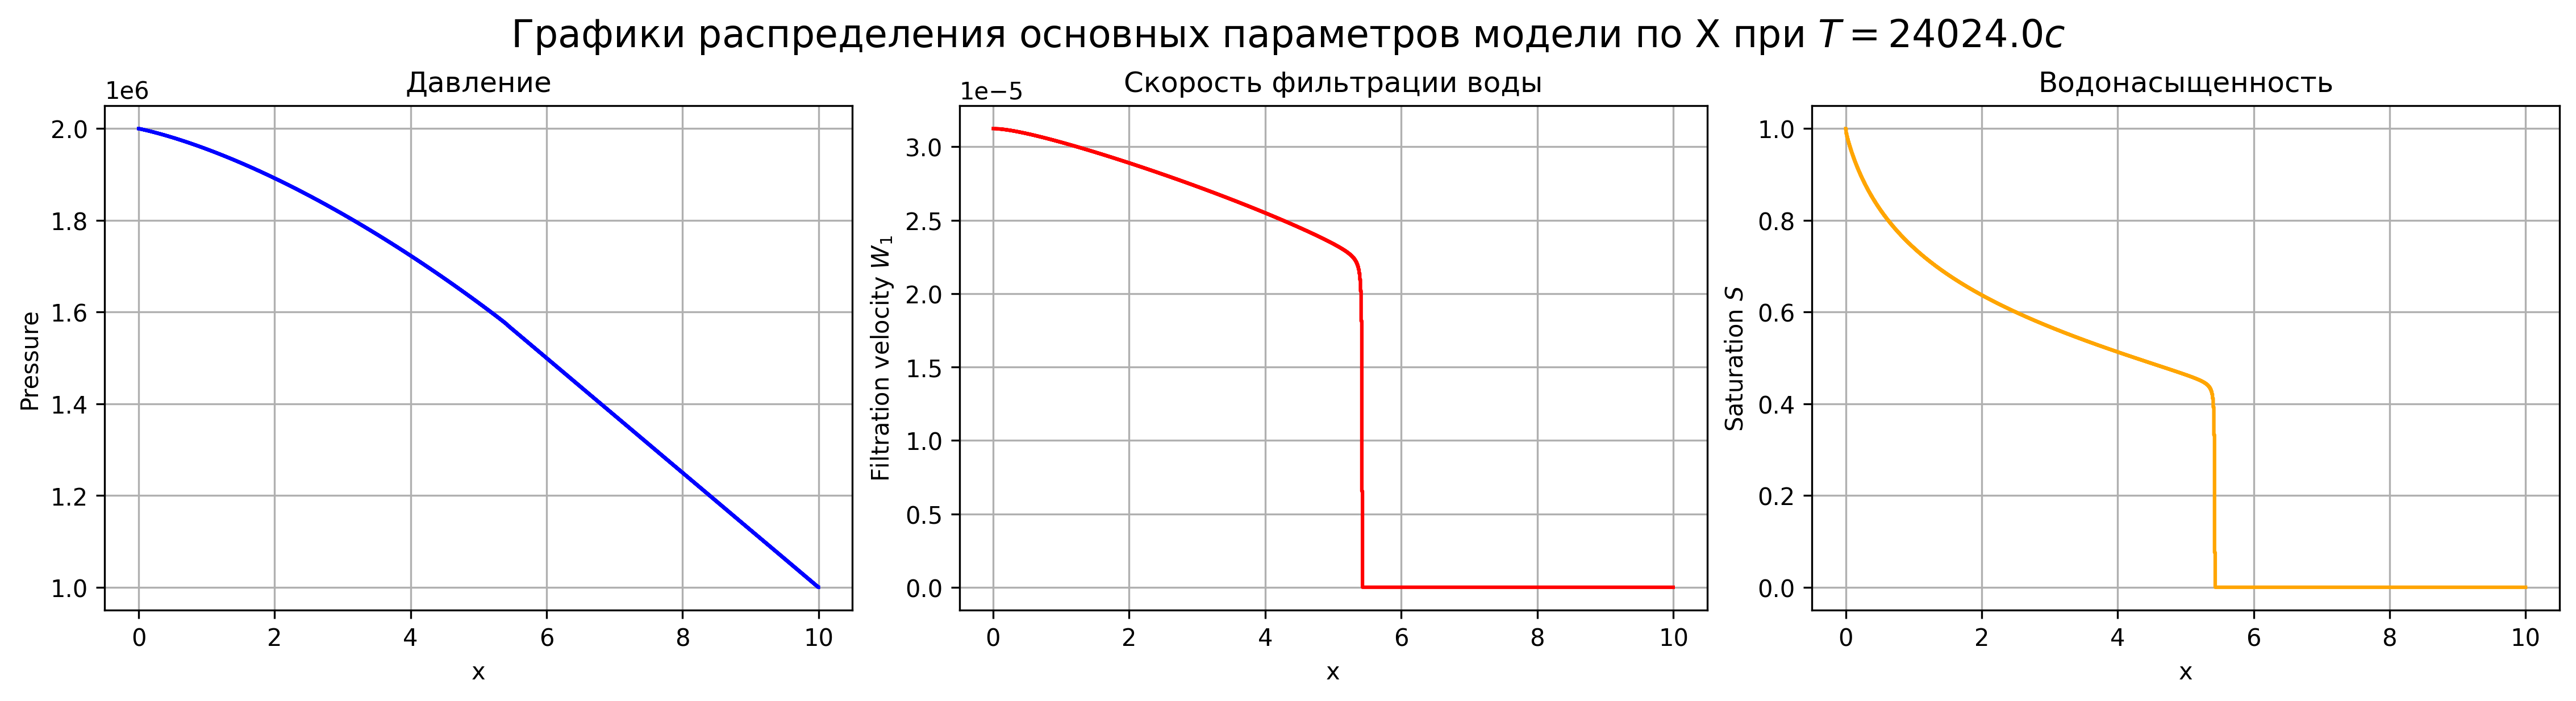
\includegraphics[width=\linewidth]{impes-params-solution.png}
    \end{figure}
    
\end{frame}

\begin{frame}
    
    \begin{figure}
        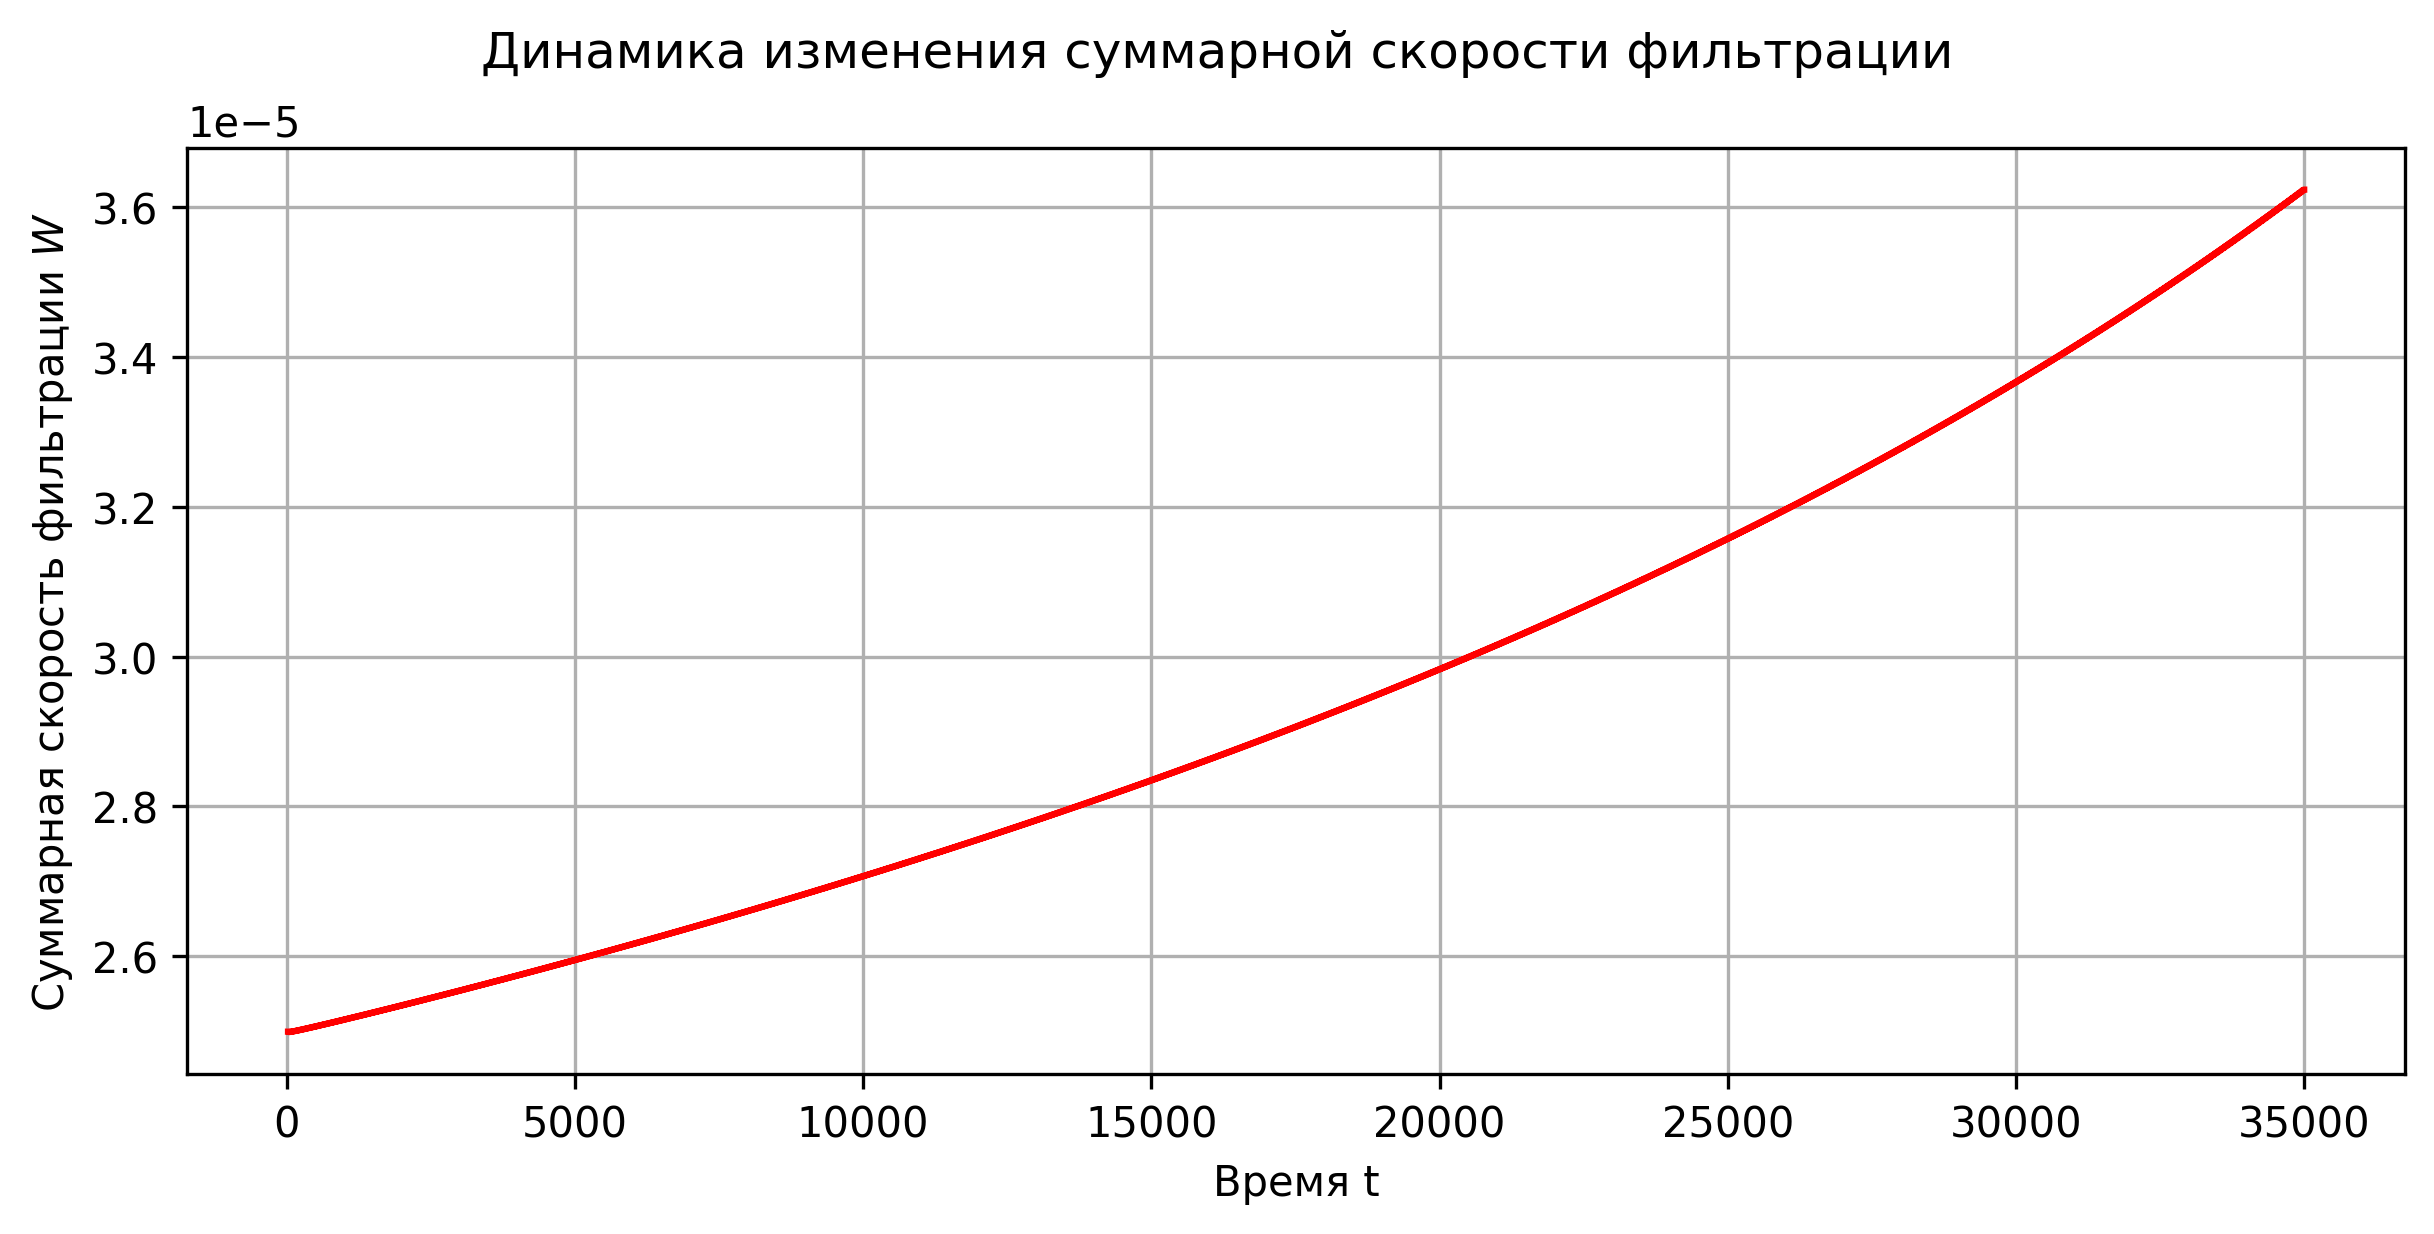
\includegraphics[width=\linewidth]{impes-velocity-time.png}
    \end{figure}
    
\end{frame}

\section{Результаты}

\begin{frame} {Сравнение результатов}

    \begin{figure}
        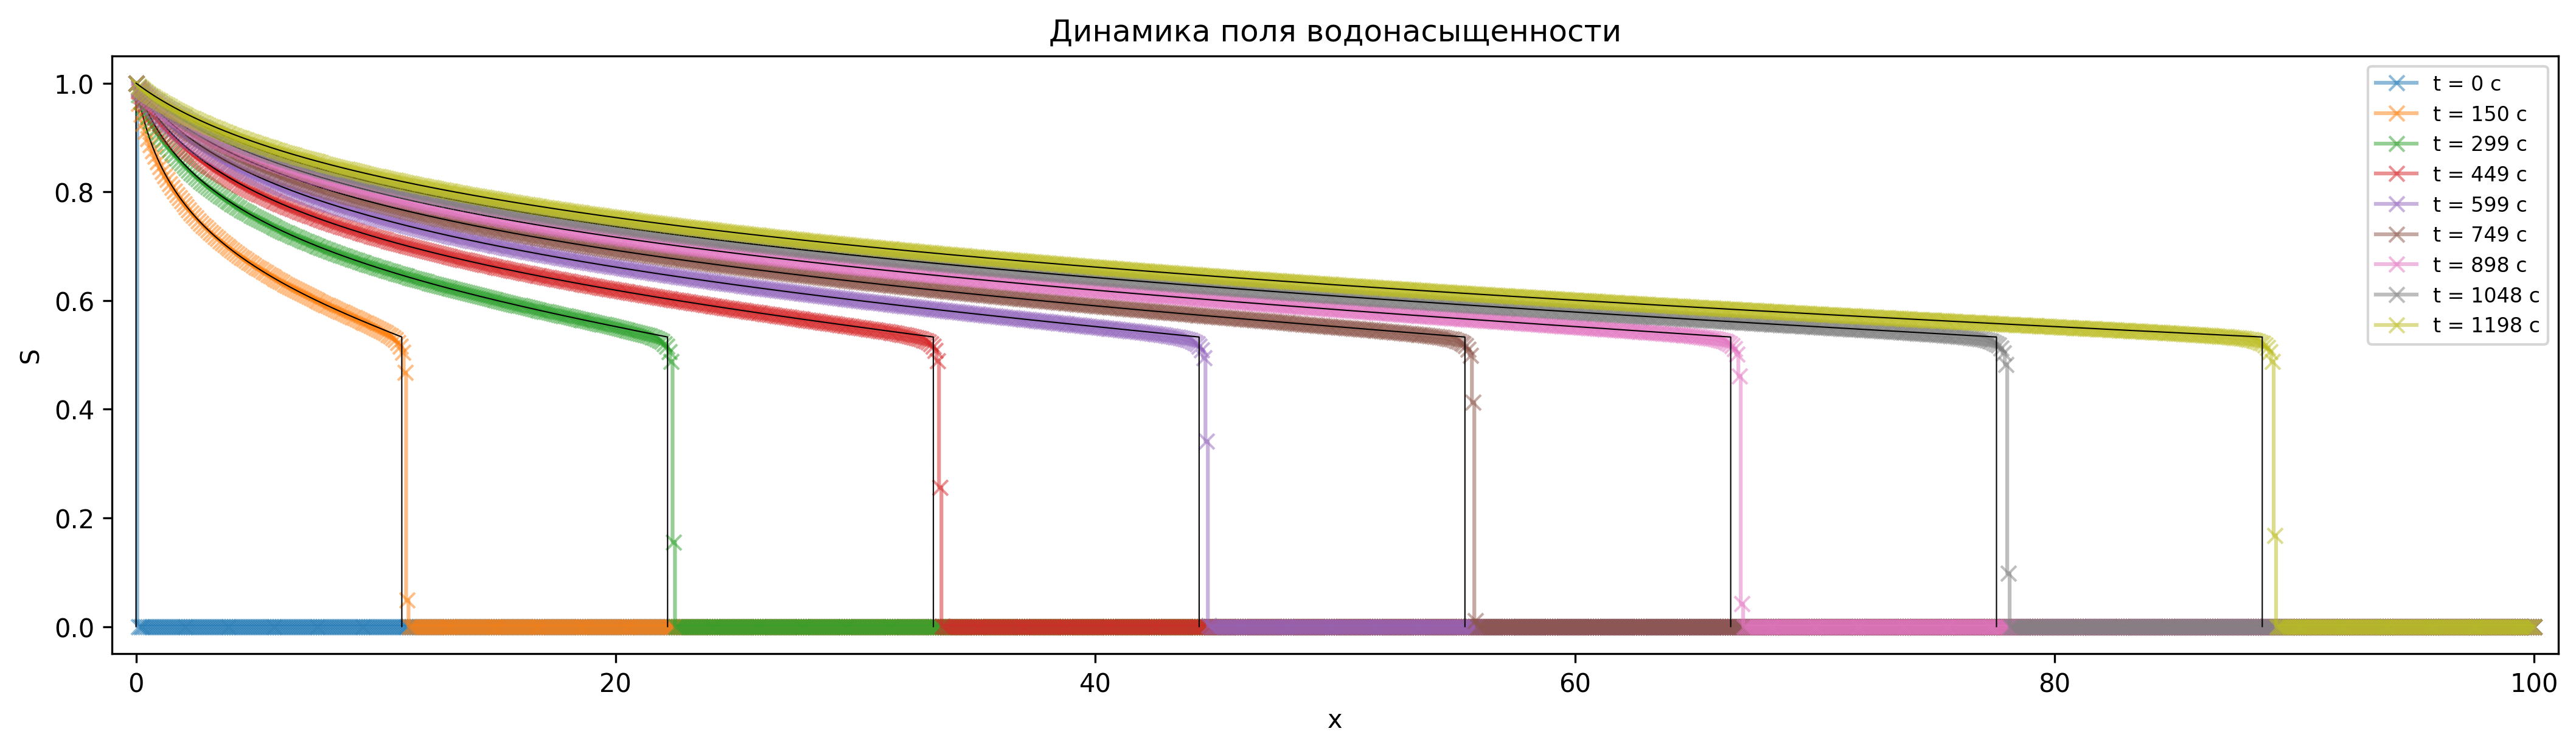
\includegraphics[width=\linewidth]{upwind-solution.png}
        \caption{Поле водонасыщенности в разные моменты времени при $W=$ const}
    \end{figure}
    
\end{frame}

\begin{frame} {Сравнение результатов}

    \begin{figure}
        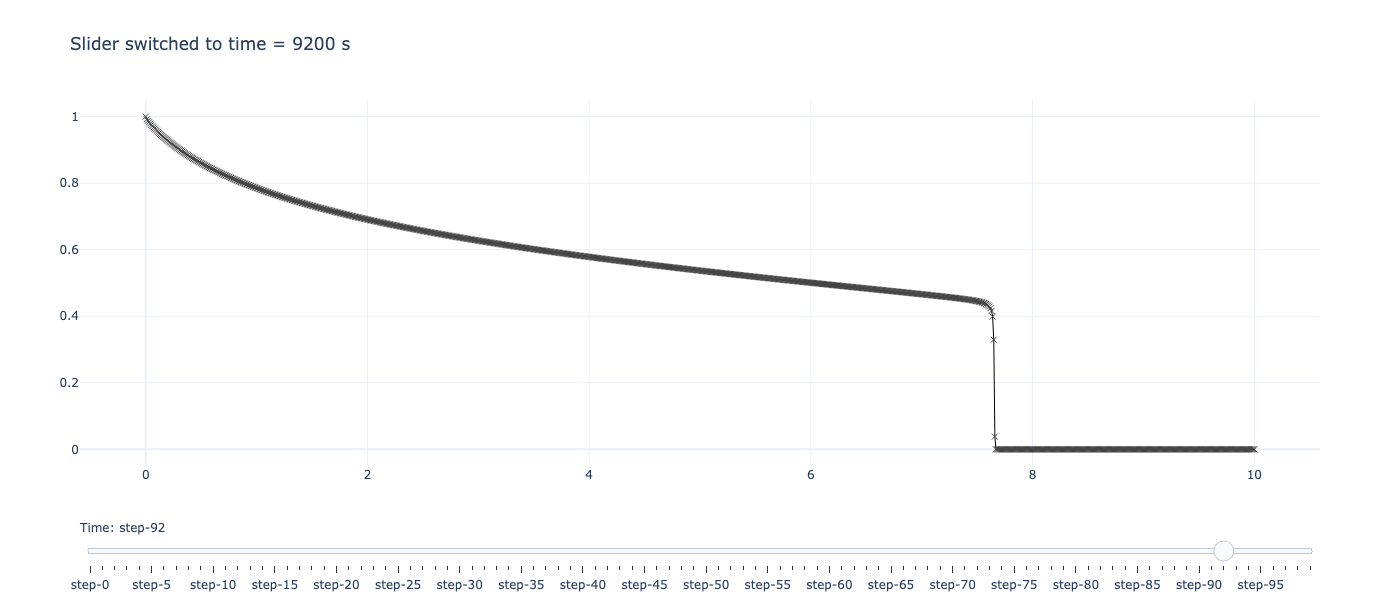
\includegraphics[width=.9\linewidth]{impes-solution.png}
        \caption{Поле водонасыщенности при $P_{bottom}=$ const}
    \end{figure}
    
\end{frame}

\section{Выводы}

\begin{frame} {Выводы}

    \begin{enumerate}
        \item Решена численно задача двухфазной фильтрации Баклея-Леверетта в одномерной постановке с граничными условиями 1-го и 2-го рода,
        \item Разработана база для дальнейшего моделирования переноса кислоты и кислотного растворения пористой среды.
    \end{enumerate}

\end{frame}

\end{document}